% !TeX spellcheck = en
\chapter{Implementation and experiments}
\label{sec:imp}

Here some code for my super neural network. 
The artificial neural networks discussed in this text are only remotely related to their biological counterparts. In this section we will briefly describe those characteristics of brain function that have inspired the development of artificial neural networks.

 
\begin{lstlisting}[caption={StudentFactory},captionpos=b]
class StudentFactory(DjangoModelFactory):
	class Meta:
		model = Student
	student_card = factory.SubFactory(StudentCardFactory)
	first_name = factory.Faker('first_name')
	second_name = factory.Faker('last_name')
\end{lstlisting}

\begin{wrapfigure}{l}{0.55\textwidth}
	\fbox{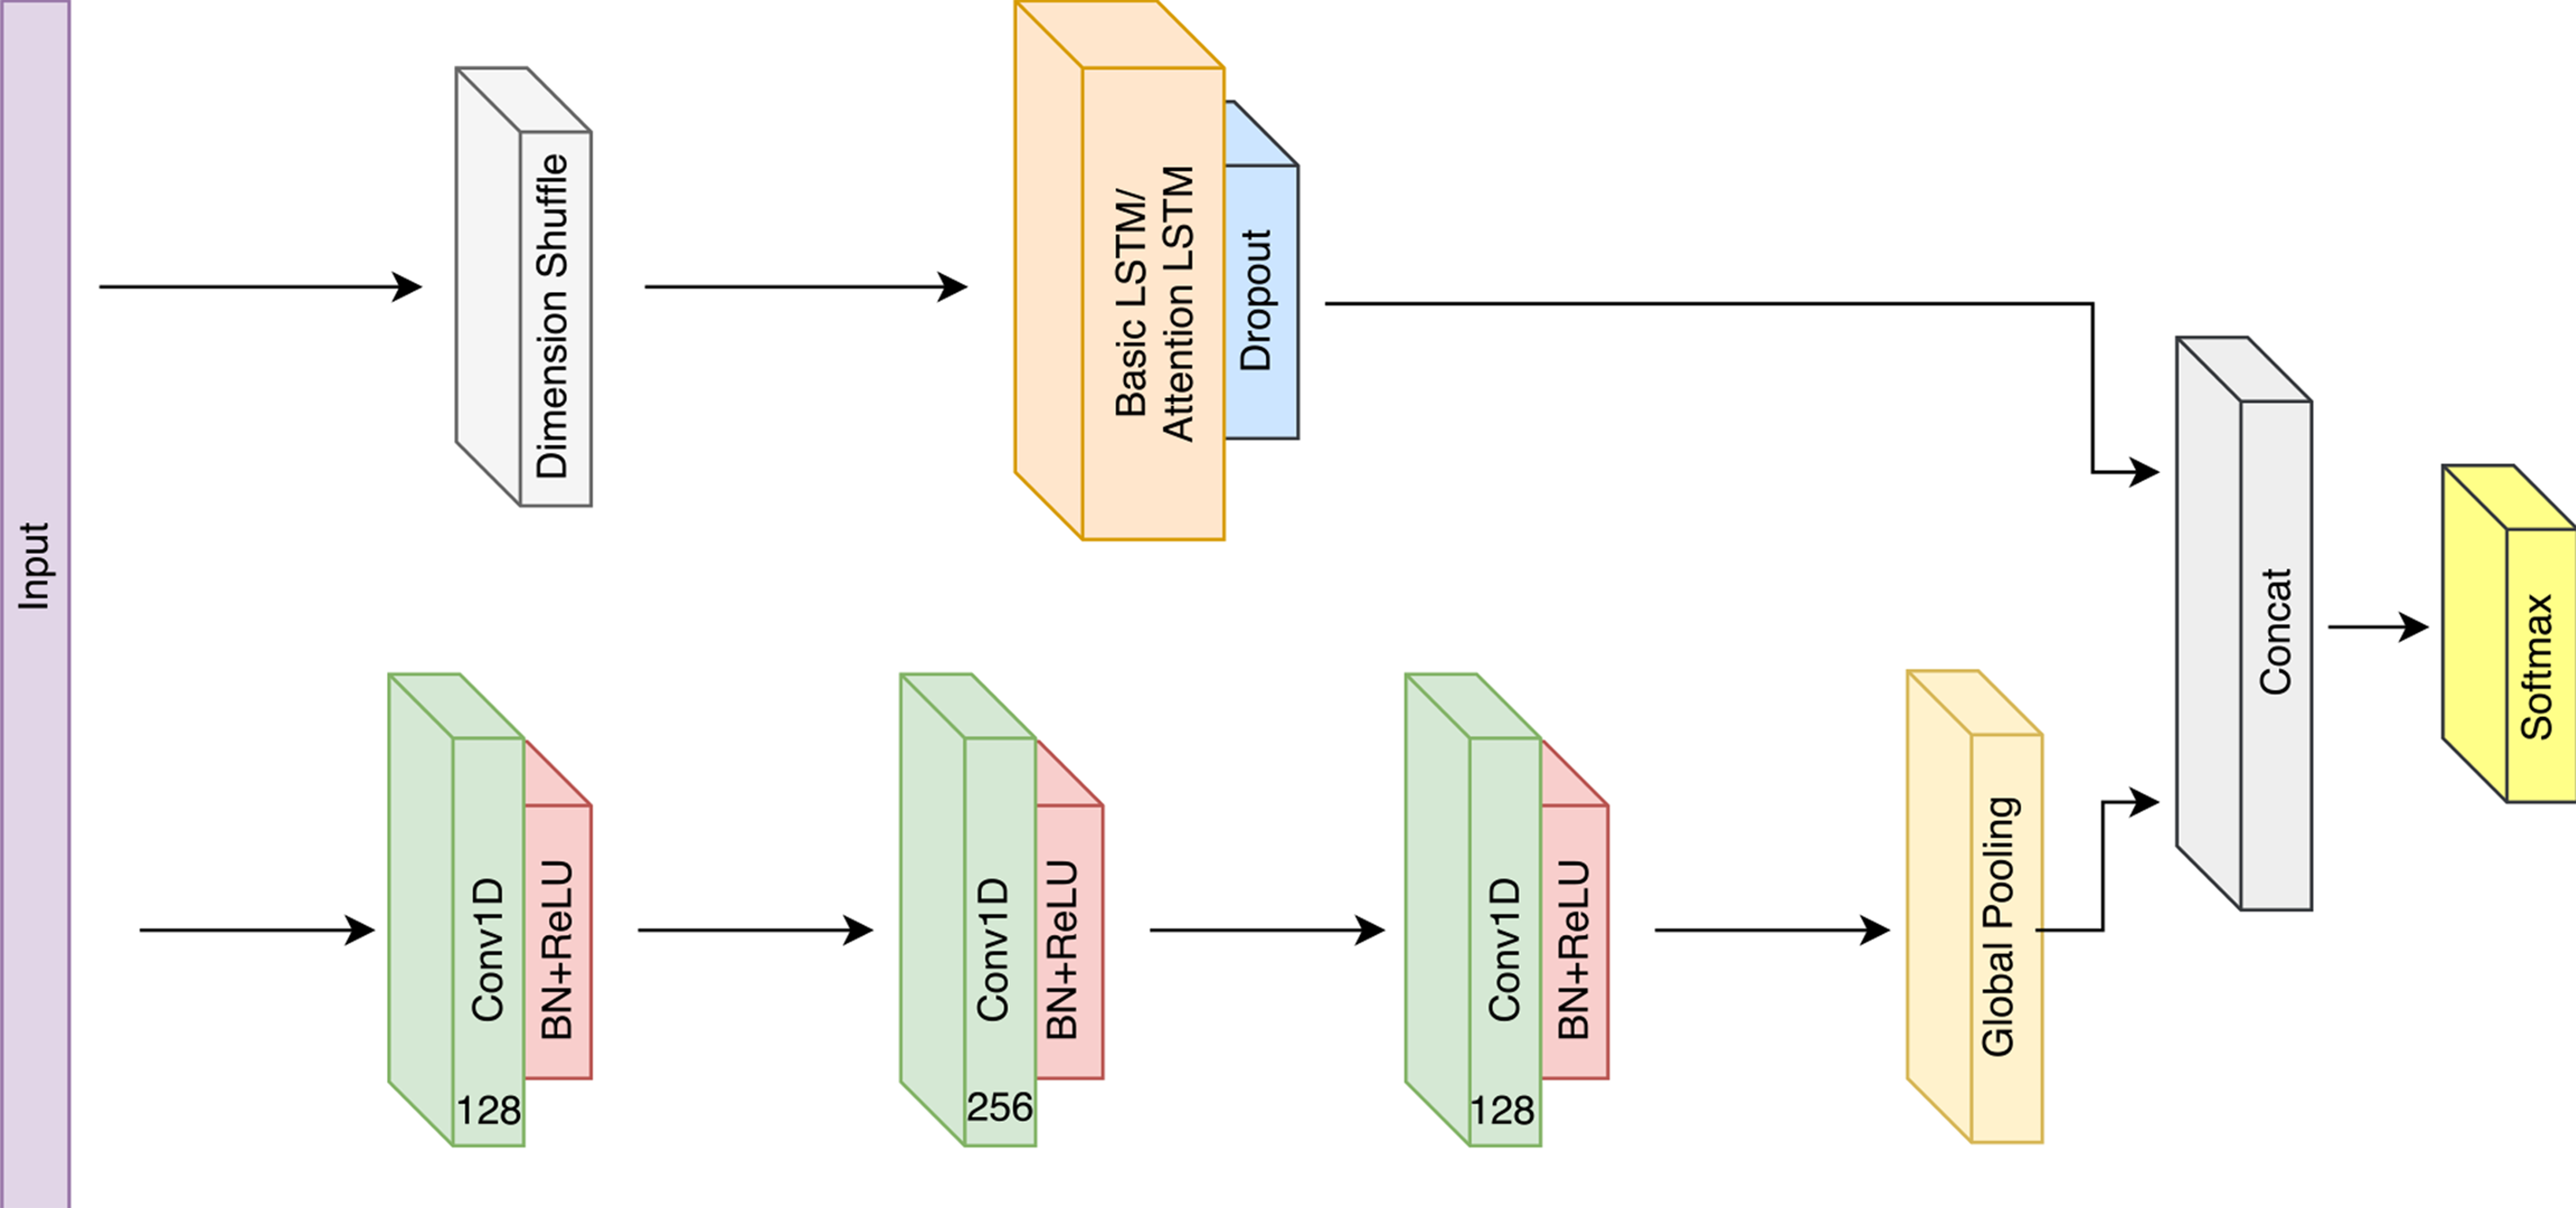
\includegraphics[width=0.5\textwidth]{gfx/LSTM-FCN.png}}
	\caption{LSTM Fully Convolutional Networks for Time Series Classification}
	\label{fig:nn1}
\end{wrapfigure}

You might already know that you want to apply an established theory or set of theories to a specific context (for example, reading a literary text through the lens of critical race theory, or using social impact theory in a market research project). 

\section{Implementation}
\label{sec:imp:programming}

\section{Experiments}
\label{sec:imp:experiments}


\section{Evaluation metrics}
\label{sec:imp:eval}


\begin{figure}
	\centering
	\fbox{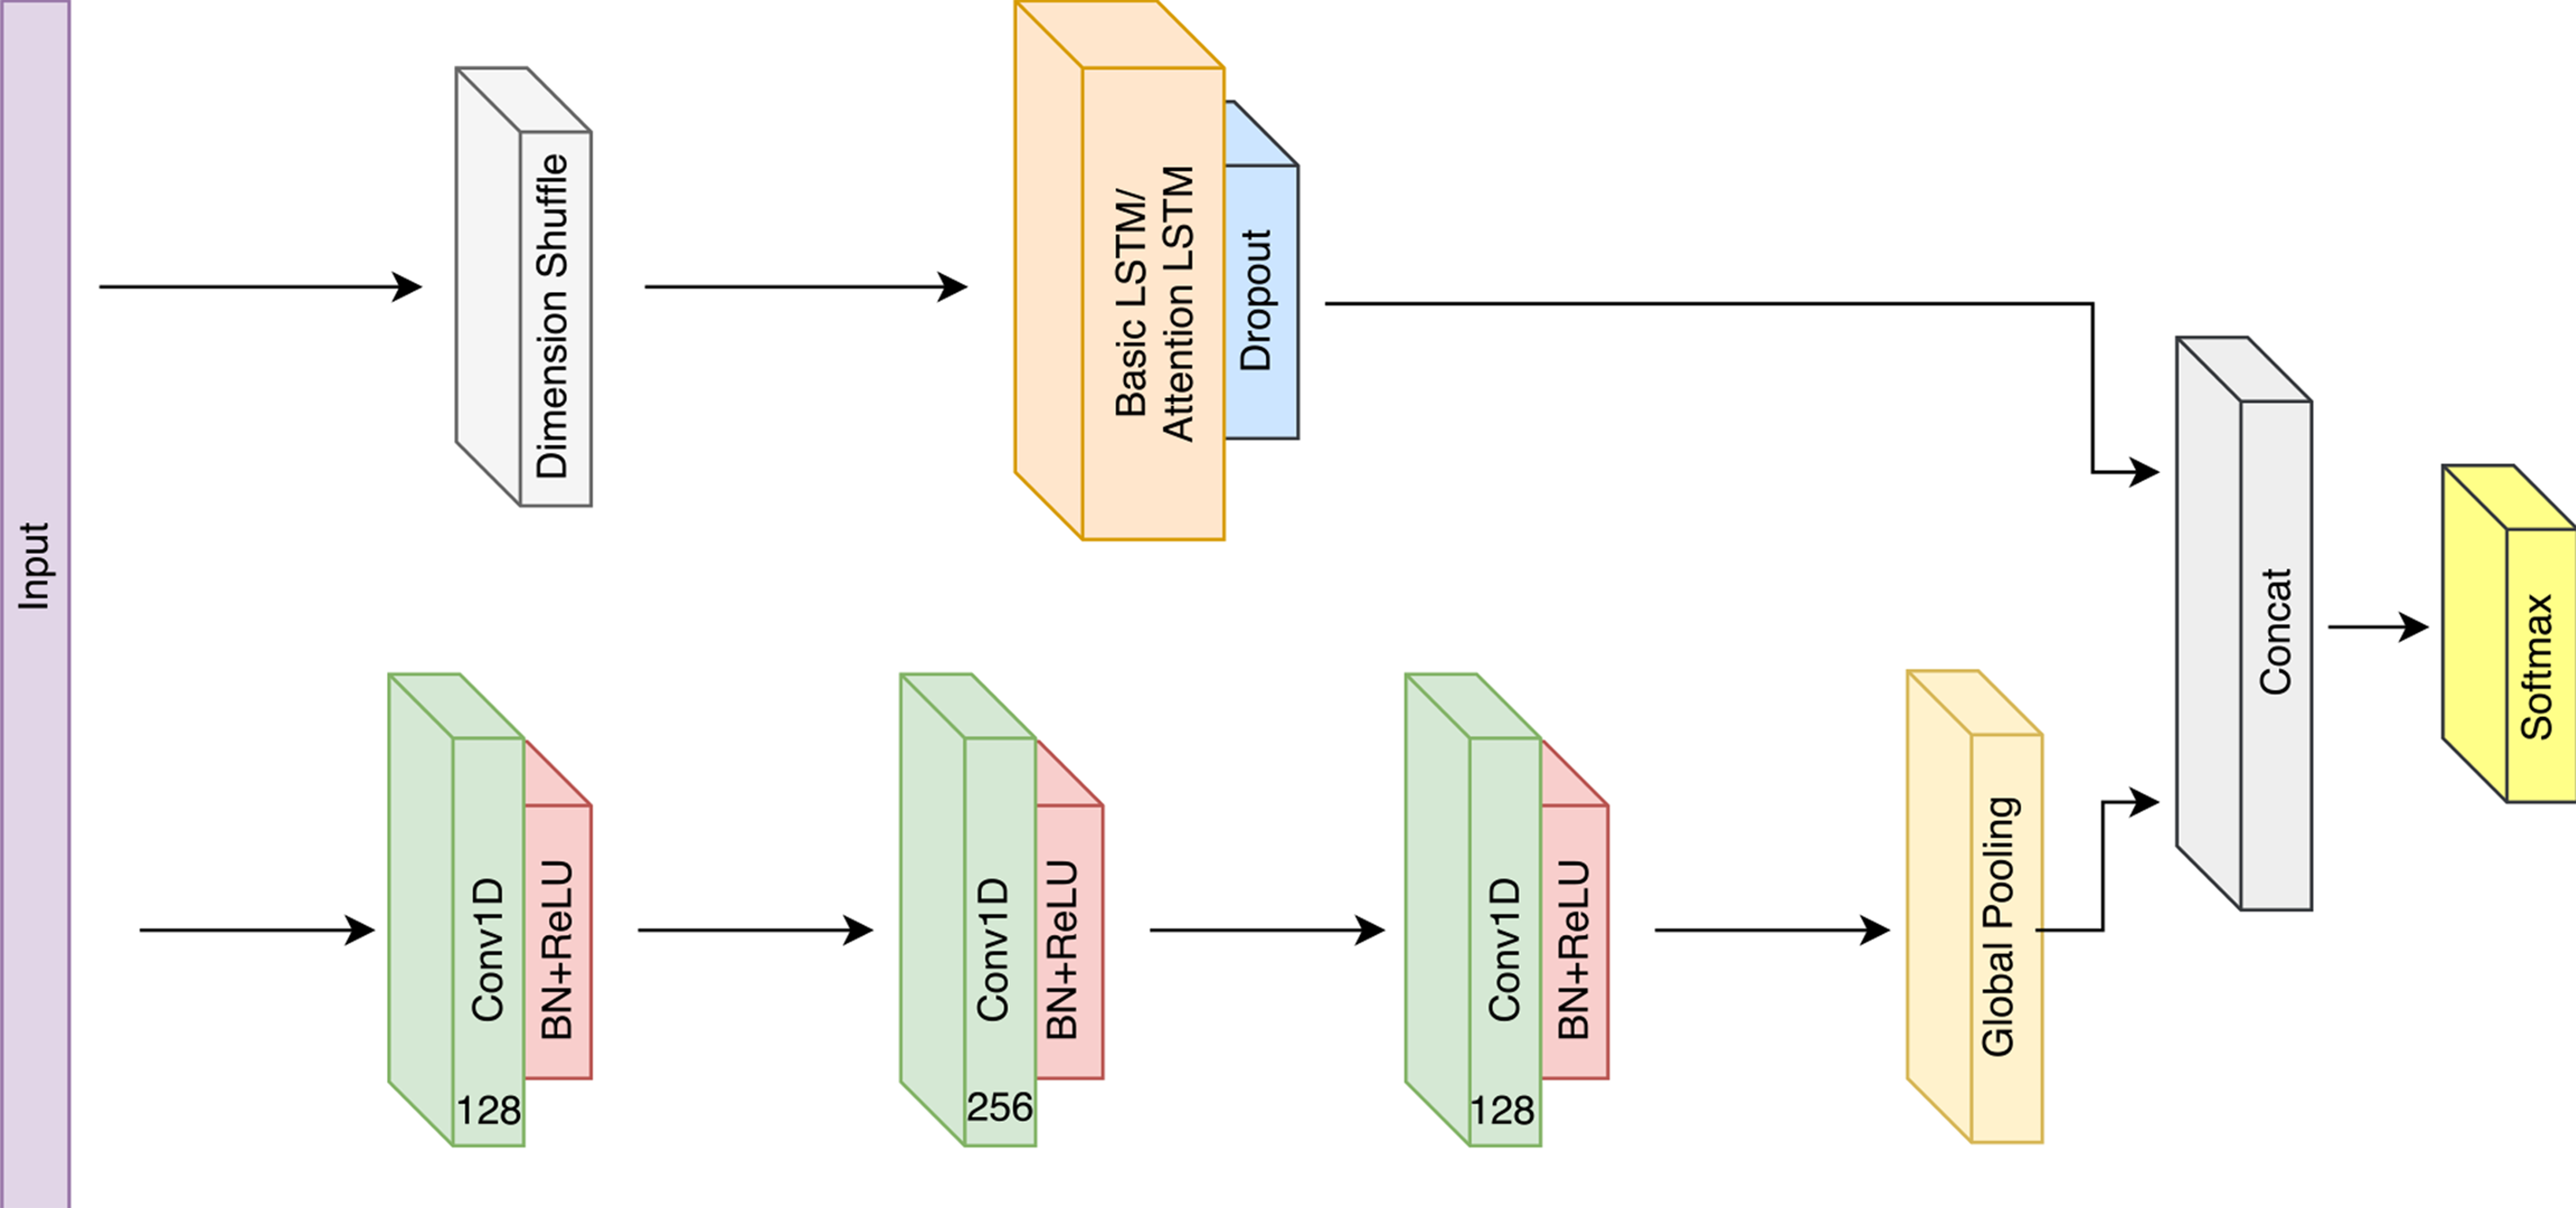
\includegraphics[width=1\textwidth]{gfx/LSTM-FCN.png}}
	\caption{LSTM FCN WRAP}
	\label{fig:nn2}
\end{figure}


\section{Results}
\label{sec:imp:results}
